\section{Method details}


% \begin{figure*}[!ht]
% \centering
% \begin{subfigure}{1.0\textwidth}
%   \centering
%   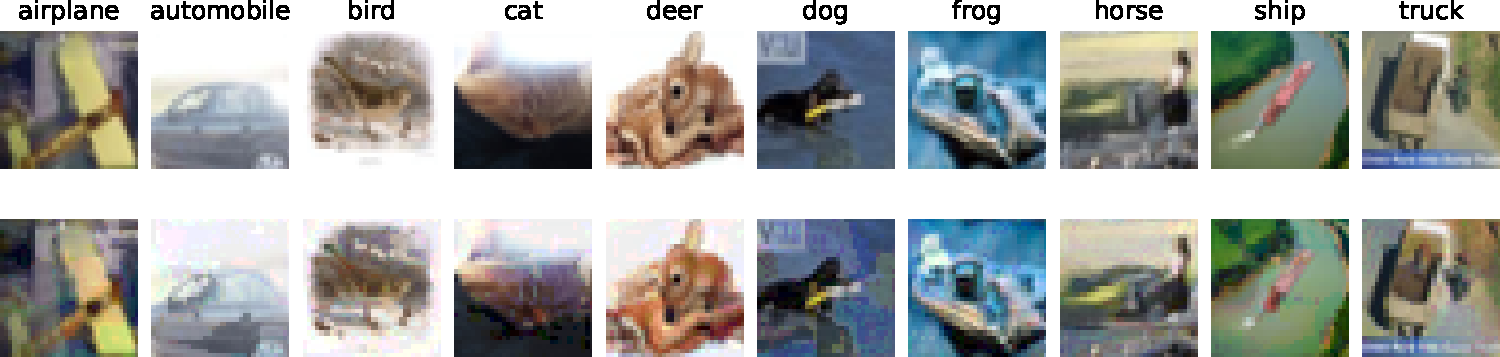
\includegraphics[width=0.95\linewidth]{figures/examples-low-quality.pdf}
%   \caption{Examples with the lowest quality and their corresponding adversarial examples.}
%   \label{fig:problematic-examples-orig}
% \end{subfigure}
% \begin{subfigure}{1.0\textwidth}
%   \centering
%   \includegraphics[width=0.95\linewidth]{figures/examples-high-quality.pdf}
%   \caption{Examples with the highest quality and their corresponding adversarial examples.}
%   \label{fig:problematic-examples-ad}
% \end{subfigure}
% \caption{Examples with the lowest and highest quality identified in the training set of CIFAR-10. In each subfigure, the top row shows the original image and the bottom row shows the image after the adversarial perturbation (PGD-10 with perturbation radius $8/255$). For each image, the true label is annotated on the top.
% % , and the predicted label is annotated on the bottom.}
% }
% \label{fig:examples}
% \end{figure*}

% Figure \ref{fig:examples} show the examples with the highest quality and lowest quality from each class. We note that the majority of those examples with poor quality are not label noise and are at most ambiguous from the human perspective. 
% A recent study also shows that noisy labels are still scarce in relatively small datasets such as CIFAR-10~\citep{Northcutt2021PervasiveLE}. % \chengyu{this is for testset, find another citation for training set}



% \subsection{Bias-variance decomposition of the 0-1 loss}
% \label{sect:bias-variance-0-1loss}
% As the double descent is typically presented in terms of the accuracy/error, we conduct a bias-variance decomposition of the 0-1 loss (equivalent to the error) to show the variance is increased by the (implicit) label noise.
% We follow the standard practice for bias-variance decomposition of the 0-1 loss~\citep{Domingos2000AUB}, where the main prediction is defined as the mode, namely the most frequent prediction, the bias is defined as the loss of the main prediction, and the variance is defined as the average loss with respect to the main prediction. We implement the decomposition based on Mlxtend~\citep{raschkas_2018_mlxtend}. We train models on $5$ independent subsets of size $5000$ randomly sampled from the training set.




\subsection{Determine the optimal hyper-parameters}
\label{sect:confidence-calibration-assigned}

% \todo{Smooth it a little bit.}

% \smallsection{Confidence calibration for adversarial training}
% For adversarial training, we calculate the NLL loss on the validation set under adversarial attack. We employ the same adversarial attack as the one used in adversarial training. We note that even if the adversarial perturbation is randomly initialized (follow a uniform distribution in our implementation), the optimal temperature and interpolation ratio are quite stable over multiple random starts. Therefore we only perform the calibration once. 


% \smallsection{Confidence calibration with assigned label}

% \todo{Algorithm description: Accuracy-constrained confidence calibration.. ($90\%$)}

% \begin{algorithm}[hbt!]
% \caption{Calibration of model probability with error constraint (used in section 4)}
% \label{alg:calibration-acc}
% \SetKwInOut{Input}{Input}
% \SetKwInOut{Output}{Output}
% \Input{$\mathcal{D}_{\text{val}}$, $f$, $f^s$, $\mathcal{D}_{\text{Train}}$, $e_{\text{th}}$}
% \Output{$T$, $\lambda$}
% \For{$x_i$, $y_i$ in $\mathcal{D}_\text{val}$}{
%     $\delta \gets \argmax_\delta \ell(f(x_i+\delta), y_i)$\;
%     $z_i \gets g_f (x_i+\delta)$\;
%     $\delta \gets \argmax_\delta \ell(f^s(x_i+\delta), y_i)$\;
%     $z^s_i \gets g_{f^s} (x_i+\delta)$\;
% }
% $T, \lambda \gets \argmin_{T, \lambda} \sum_i~\ell\left(\lambda\cdot \softmax(z_i / T) + (1-\lambda)\cdot\softmax(z_i^s/T), y\right)$, $e(\mathcal{D}_\text{train}; T, \lambda) > e_{\text{th}}$\;
% \end{algorithm}


% The algorithm to search the optimal temperature and interpolation ratio

% \begin{algorithm}[hbt!]
% \caption{Calibration of model probability}
% \label{alg:calibration}
% \SetKwInOut{Input}{Input}
% \SetKwInOut{Output}{Output}
% \Input{$\mathcal{D}_{\text{val}}$, $f$, $f^s$}
% \Output{$T$, $\lambda$}
% \For{$x_i$, $y_i$ in $\mathcal{D}_\text{val}$}{
%     $\delta \gets \argmax_\delta \ell(f(x_i+\delta), y_i)$\;
%     $z_i \gets g_f (x_i+\delta)$\;
%     $\delta \gets \argmax_\delta \ell(f^s(x_i+\delta), y_i)$\;
%     $z^s_i \gets g_{f^s} (x_i+\delta)$\;
% }
% $T, \lambda \gets \argmin_{T, \lambda} \sum_i~\ell\left(\lambda\cdot \softmax(z_i / T) + (1-\lambda)\cdot\softmax(z_i^s/T), y\right)$
% \end{algorithm}


One may note that Equation~(\ref{eq:calibration}) cannot be directly optimized since the traditional adversarial label is only defined on the example in the training set and cannot be simply generalized to the validation set.
A reasonable solution is using the nearest neighbour classifier to find the closest traditional adversarial label for every example in the validation set. 
% will degenerate to $\lambda=0$ since the traditional adversarial label happens to the same as the  leads to a degeneration since the NLL loss of the true label is always 0. (\note{What is the root cause of this problem? Because the true label leaks in the construction of label}) 
However, to speed up the optimization, we propose to employ the classifier overfitted by the traditional adversarial labels on the training set as an surrogate, which works well in practice.
% To automatically tune the temperature $T$ and the interpolation ratio $\lambda$, we employ the NLL loss on the validation set as mentioned in Section~\ref{sect:synthetic} to automatically determine the optimal values of $T$ and $\lambda$. 
Specially, we employ a model overfitted on the training set to generate approximate traditional adversarial label of the adversarial example in the validation set. Such overfitted model is typically the model at the final checkpoint when conducting regular adversarial training for sufficient epochs. Mathematically, our final method to determine the optimal temperature and interpolation ratio in rectified model probability can be described as
\begin{equation}
    T, \lambda = \argmin_{T, \lambda} \mathbbm{E}_{(x', y')\sim \mathcal{D}'_\text{val}}~\ell\left(\lambda\cdot f_\theta(x'; T) + (1-\lambda)\cdot f_{\theta_s}(x'; T), y'\right),
\end{equation}
where $f_{\theta_s}(x'; T)$ denotes the temperature-scaled predictive probability of a surrogate model on $x'$. Here the validation set is constructed by applying adversarial perturbation generated by $f_\theta$ to the clean validation set. For adversarial perturbation we utilize PGD attack with $10$ iterations, the perturbation radius as $8/255$ and the step size as $2/255$.
Note that Such process incurs almost no additional computation as we simply obtain the logits of a surrogate classifier. %  on the validation set. 

% \begin{equation}
%     T, \lambda = \argmin_{T, \lambda} \mathbbm{E}_{(x, y)\sim \mathcal{D}_\text{val}}~\ell\left(\lambda\cdot\frac{\vec{z}(x+\delta)/T}{\sum_k \exp(z_j(x+\delta)/T)} + (1-\lambda)\cdot\frac{\vec{z^s}(x+\delta)/T}{\sum_k \exp(z^s_j(x+\delta)/T)}, y\right)
% \end{equation}

% \begin{equation}
%     \label{eq:calibration}
%     T, \lambda = \argmin_{T, \lambda} - \mathbbm{E}_{(x_\delta, y_\delta^*)\in \mathcal{D}_\delta^\text{val}} \log p_{\theta; T, \lambda} (y_\delta = y^*_\delta | x_\delta) 
% \end{equation}

%   \begin{equation}
%         \label{eq:approximate-label-distribution}
%         p_{\theta; T, \lambda}(y_\delta|x_\delta) = \lambda \cdot f(x_\delta; \theta, T) + (1- \lambda) \cdot p(\tilde{y}_\delta | x_\delta),
%     \end{equation}
    
    
%         $$
%         f(x; \theta, T)_j = \frac{\exp(z_j/T)}{\sum_j \exp(z_j / T)},
%     $$

% When performing the confidence calibration for an interpolation between model probability and the assigned label, we have to calculate the NLL loss of the assigned label of the training set on the validation set, which is not straightforward. To this end, we employ the model at the last checkpoint (for both the training setting in double descent and the practical training setting) as a surrogate model for the assigned label. Under sufficient training, the last model is typically overfitted, achieving $100\%$ accuracy in terms of the assigned label and the predictive probability is almost one-hot. Therefore it adequately models the assigned label. We found this strategy works well in practice to determine the optimal interpolation ratios for experiments on both mixup augmentation (Appendix~\ref{sect:better-approximate-mixup}) and adversarial training (Section~\ref{sect:exp-practical-adversarial-training}).
